\chapter{Casolysis}

\label{chap:Casolysis}

Casolysis is a free card sorting tool that was developed by multiple
students at the University of Paderborn~\parencite{Casolysis}. It is
standalone Windows .exe file that requires no installation. The tool 
is no longer under development, but can still be downloaded from the 
university's website.

Similar to \textcite{SynCaps}  offers no actual card sorting tool, but rather
takes over the analytical part of the process. Card sorting needs to
be done in some other form, be it physical or with a different tool,
and then the results can be imported to Casolysis.

\begin{figure}[tp] 
\centering
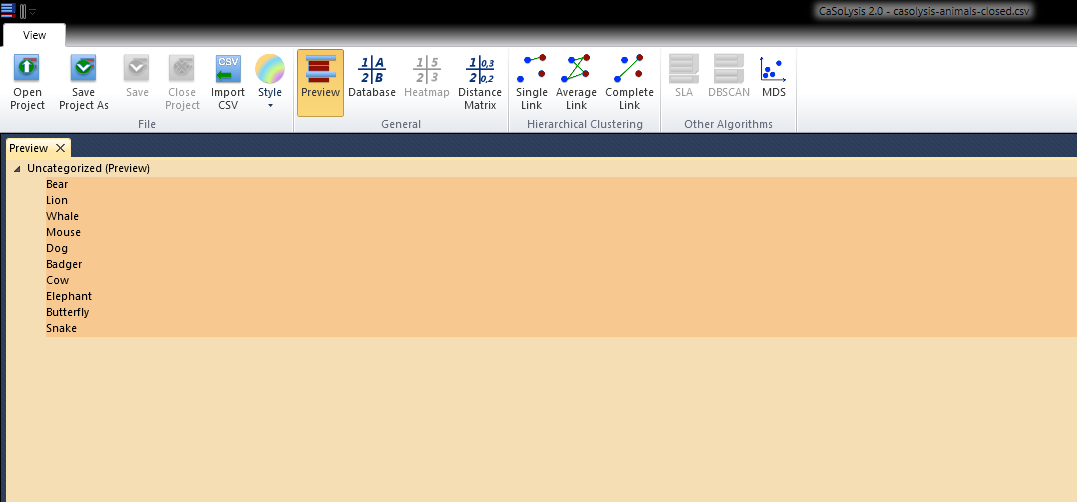
\includegraphics[keepaspectratio,width=\linewidth,height=\halfh]{images/casolysis-sorting.png}
\caption[Casolysis Application] { This is the base view within Casolysis
once data is imported with a .csv file.
\imgcredit{Screenshot was captured by Christopher Oser using
\textcite{Casolysis}.} }
\label{fig:Casolysis1}
\end{figure}

\section{Business Model}
Casolysis is free of charge and can be downloaded an unlimited amount
of times. Its development has seized, but the tool can still be used
in its current form.

Additionally no account is needed to access Casolysis. It does
not even require installation, but can be run straight out of the .exe
file.

\section{Card Sorting}
Casolysis does not support the actual sorting of cards. It needs to be
used in cooperation with another form of card sorting, be it physical
paper card sorting or a different card sorting tool. The results can
then be imported to Casolysis via a .csv file for analytics.

\section{Analytics}
The core functionality of Casolysis, analyzing card sorting results.
Once data is imported it is very simple to produce analytics. Before
the analyzing begins, it is possible to adjust the data a bit, adjusting
sources, in case the .csv file was not correctly formatted, deciding
whether the experiment was done though open or closed card sorting and
whether or not sub-categories were in use.

As soon as the data is ready, all analytics Casolysis offers are only
one button click away. Although Casolysis does not seem to have any 
kind of documentation, usage was rather simple and no documentation was
required during the review process.

The analytical visualizations are made up of a heatmap, distance
matrix , dendrograms for hierarchical clustering and 3 other
miscellaneous  algorithms. The distance map and a dendrogram can be
seen in Figures~\ref{fig:Casolysis2} and \ref{fig:Casolysis3}
respectively.With all these possibilities, lots of knowledge can be
extracted from experiment results.

The features are summarized in Table~\ref{tab:features-Casolysis}.

\begin{figure}[tp] 
\centering
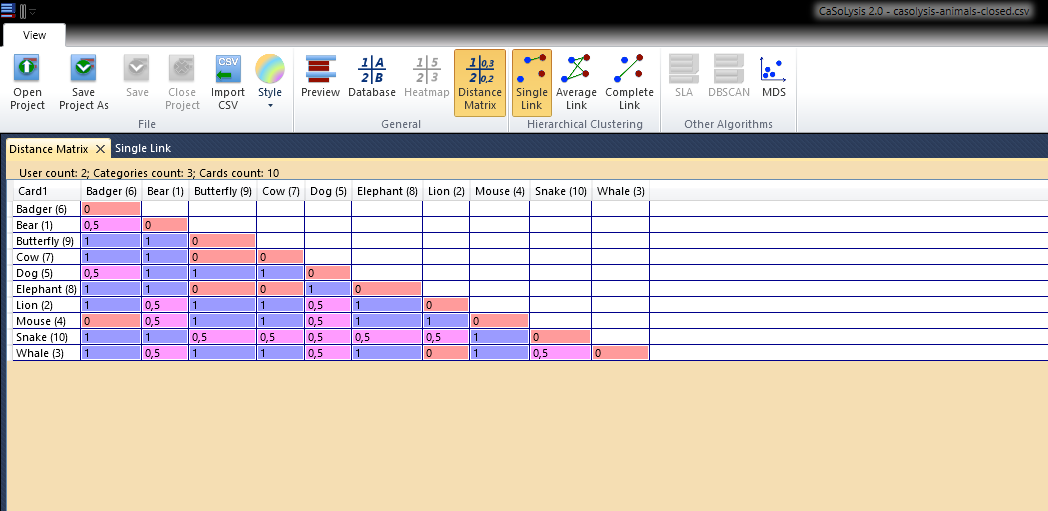
\includegraphics[keepaspectratio,width=\linewidth,height=\halfh]{images/casolysis-diagram-1.png}
\caption[Casolysis Distance Matrix] { This screenshot shows a distance
matrix over all cards that is used for analytics.
\imgcredit{Screenshot was captured by Christopher Oser using
\textcite{Casolysis}.} }
\label{fig:Casolysis2}
\end{figure}

\begin{figure}[tp] 
\centering
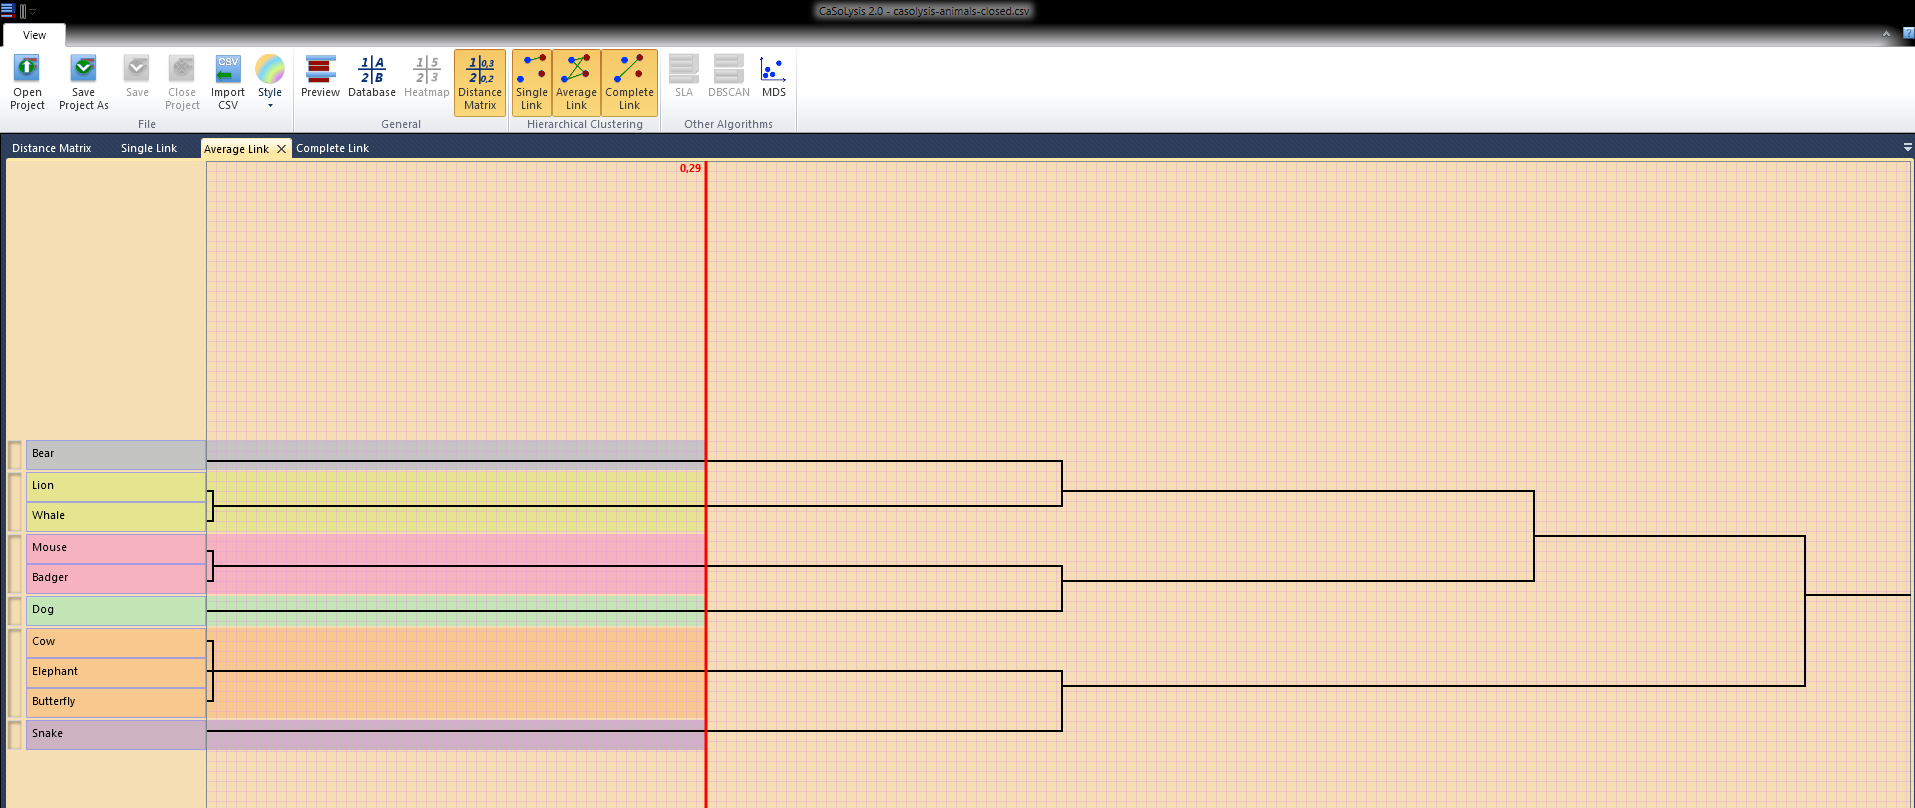
\includegraphics[keepaspectratio,width=\linewidth,height=\halfh]{images/casolysis-diagram-2.png}
\caption[Casolysis Dendrogram] { This screenshot shows a dendrogram 
for the average link of cards which is used for analytics.
\imgcredit{Screenshot was captured by Christopher Oser using
\textcite{Casolysis}.} }
\label{fig:Casolysis3}
\end{figure}

\begin{table}[tp]
\centering
\begin{tabularx}
{\linewidth}{|l|X|}
\hline \textbf{Feature/Characteristic} & \textbf{Availability in Casolysis} \\ 
\hline Card Sorting & None. Paper Cards or other tools needed. \\ 
\hline Card Limit & None. \\
\hline Participant Limit & None. \\
\hline Analytics & Analytics with 5 different types of visualizations
with different versions for some of them. \\ 
\hline Documentation & None. \\
\hline Business Model & Free. No longer under development \\
\hline Import formats & .csv\\ 
\hline Export formats & None. Screenshots of visualizations possibly. \\ 
\hline Sub-Categories & Yes, sub-categories are supported \\ 
\hline Playback of user-sessions & No. \\ 
\hline Data preparation & Very little - open/closed and sub-categories.
Everything else must be done manually. \\ 
\hline
\end{tabularx} 
\caption[Feature summary of Casolysis] 
{ 
This table summarizes all the features and characteristics of Casolysis
to provide an easy to read overview.
}
\label{tab:features-Casolysis}
\end{table}


\section{Summary \& Ratings}
All in all Casolysis seems to be a more modern \textcite{SynCaps},
minus the extensive data preparation options. Nevertheless it offers
more analytics and does so in a much simpler way. The visualizations
are easy to understand and frankly, quite pleasing to the eye.

Since its development has ended, there will be no added features in
the future and any bugs that might occur will not be fixed. So this
should be taken into account when considering Casolysis.

If the features are sufficient and you do not require card sorting
capabilities the tool seems to be a great fit. The only final drawback
being, that it is offline and needs Windows to be run.


\begin{table}[tp] 
\centering 
\begin{tabularx}{\linewidth}{|X|X|X|X|X|}
\hline
Simplicity & Documentation & Features & Business Model & Average \\ 
\hline 
4 & 0 & 4 & 5 & 3.25 \\ 
\hline 
\end{tabularx} 
\caption[Ratings for Casolysis] {
Ratings for Casolysis including the average rating.
} 
\label{tab:rating-Casolysis}
\end{table}